% % igs2eguide.tex
% % v2.00 12-jun-08
% 
% % \NeedsTeXFormat{LaTeX2e}
% 
% % The default is for Journal of Glaciology, one column, A4 paper. The other options are listed below:
% 
% %\documentclass{igs}
% %   \documentclass[twocolumn]{igs}
% % \documentclass[annals]{igs}
% % \documentclass[annals,twocolumn]{igs}
% 
% % \documentclass[letterpaper]{igs}
% % \documentclass[twocolumn,letterpaper]{igs}
% % \documentclass[annals,letterpaper]{igs}
% % \documentclass[annals,twocolumn,letterpaper]{igs}
% 
% % when submitting your article for review, use one
% % of the following two options:
% 
% % \documentclass[review]{igs}
% % \documentclass[review]{igs}
% 
% % \documentclass[annals,review]{igs}
% 
%   \usepackage{igsnatbib}
%   \usepackage{stfloats}
% 
% % check if we are compiling under latex or pdflatex
%   \ifx\pdftexversion\undefined
%     \usepackage[dvips]{graphicx}
%   \else
%     \usepackage[pdftex]{graphicx}
%   \fi
% 
% \usepackage[T1]{fontenc}
% \usepackage{lmodern} %this is needed with T1
% \usepackage[utf8]{inputenc}  
% % the default is for unnumbered section heads
% % if you really must have numbered sections, remove
% % the % from the beginning of the following command
% % and insert the level of sections you wish to be
% % numbered (up to 4):
% 
% % \setcounter{secnumdepth}{2}
% 
% \begin{document}

% \chapter[Tidally-driven ice speed variation at Helheim Glacier, Greenland observed with terrestrial radar interferometry ]{Tidally-driven ice speed variation at Helheim Glacier, Greenland observed with terrestrial radar interferometry \footnote{This chapter is in press as: Voytenko, D., Stern, A., Holland, D. M., Dixon, T. H., Walker, R. T., Christianson, K., (2015), 
% Tidally-­driven ice speed variation at Helheim Glacier, Greenland observed with Terrestrial Radar Interferometry, Journal of Glaciology.
% }}
% 
% \chapter{He}

\chapter[InSAR Monitoring of Ground Deformation Due to CO$_{2}$ injection at an Enhanced Oil Recovery Site, West Texas]{InSAR Monitoring of Ground Deformation Due to CO$_{2}$ injection at an Enhanced Oil Recovery Site, West Texas \footnote{This chapter has been reprinted from the International Journal of Greenhouse Gas Control with permission as: Yang, Q., Zhao, W. L., Dixon, T. H., Amelung, F., Han, W. S., Li, P., (2015), InSAR Monitoring of Ground Deformation Due to CO$_{2}$ injection at an Enhanced Oil Recovery Site, West Texas, International Journal of Greenhouse Gas Control, 41, 20-28.}}

% 
% \author[Voytenko and others]{Denis VOYTENKO,$^1$ Alon STERN,$^2$ David M. HOLLAND,$^2$ Timothy H. DIXON,$^1$ Knut CHRISTIANSON,$^2$ Ryan T. WALKER$^{3,4}$}
% 
% \affiliation{%
% $^1$School of Geosciences,
% University of South Florida, Tampa, Florida, USA.\\
% E-mail: qianyang@mail.usf.edu\\
% $^2$Courant Institute of Mathematical Sciences, New York University, New York, New York, USA\\
% $^3$Cryospheric Sciences Laboratory, NASA Goddard Space Flight Center, Greenbelt, Maryland, USA\\
% $^4$Earth System Science Interdisciplinary Center, University of Maryland, College Park, Maryland, USA
% }

\section{Abstract} 
Interferometric Synthetic Aperture Radar (InSAR) measurements have been used to measure ground deformation associated with fluid injection/production at an Enhanced Oil Recovery (EOR) field in Scurry County, West Texas. 100 million tons (Mt) of supercritical CO$_{2}$ have been sequestered here since 1972, of which about half has been sequestered since 2004.  InSAR data show surface uplift up to 10 cm in the field between January 2007 and March 2011.  We evaluated data concerning injection and production of CO$_{2}$, water, oil and hydrocarbon gas from 2004 to 2011 to investigate causes of the observed uplift.  An analytical model is used to calculate reservoir pressure change and surface displacement.  Our simulations show up to 10 MPa pressure buildup in the reservoir over four years of net injection and production.  Surface displacement predictions agree well with the InSAR observations.  Water injection alone cannot explain the 2007 – 2011 surface uplift because the net injected water ($\sim$1~Mt) is negligible compared to the net injected CO$_{2}$ ($\sim$24~Mt).  The predicted total pressure buildup (up to 10 MPa) consists of net CO$_{2}$ injection (up to 12 MPa), net water injection (up to 2 MPa), and oil and gas production (up to -0.4 MPa).  Hence, observed ground uplift was mainly caused by CO$_{2}$ injection.
% \maketitle


\section{Introduction}

An important aspect of large-scale Carbon Capture, Utilization and Storage (CCUS) is the ability to assess the fate of injected CO$_{2}$ and test for leakage.  These so-called Monitoring, Verification and Accounting (MVA) activities typically involve active seismic surveys and down-hole techniques for precise tracking of CO$_{2}$ plume migration, both of which can be expensive.  Since the economic viability of CCUS is impacted by the cost of MVA activities, development of lower cost approaches is desirable.

Injection of CO$_{2}$ or other fluid into a reservoir at depth increases fluid pressure in the reservoir, causing deformation in the overlying strata and inducing surface deformation.  If the pressure change is large enough, the surface deformation may be measurable.  In principle, the measured surface deformation can be inverted to estimate pressure changes at depth and track the CO$_{2}$ plume \cite[e.g.,][]{vasco2008reservoir,vasco2010satellite,rinaldi2013modeling,white2014geomechanical,karegar2015gps}.  Over long periods (decades or centuries), chemical reactions that result in formation of mineral phases will cause pressure and volume reduction and subsidence, and could not be distinguished from migration or leakage with this technique alone.  On the other hand, surface deformation can be measured at relatively low cost, the interpretation is relatively straightforward, and the technique gives useful information in the critical few years immediately following injection.

Enhanced Oil Recovery (EOR) refers to techniques for increasing the amount of oil extracted at depleted or high viscosity oil fields.   CO$_{2}$-Enhanced Oil Recovery (CO$_{2}$-EOR) has been used by the oil and gas industry for over 40 years \cite[]{orr1984use}, but only recently has its potential as a promising method of carbon sequestration been realized and investigated \cite[]{bryant2007geologic}.  Considering the potential of CO$_{2}$-EOR for implementation of large-scale carbon emission reduction \cite[]{metz2005carbon}, it is important to test surface deformation MVA techniques in a CO$_{2}$-EOR field.

Interferometric Synthetic Aperture Radar (InSAR) technique has been successfully used to monitor surface deformation associated with CO$_{2}$ injection at the In Salah field in Algeria \cite[]{mathias2009approximate,morris2011study,shi2012assessment,verdon2013comparison}.  In this paper, we use InSAR to study surface deformation associated with a CO$_{2}$-EOR project in West Texas.  We use an analytical model and historical injection and production data to estimate CO$_{2}$ plume extent and reservoir pressure change constrained by surface deformation observations. The study reveals that ground uplift between January 2007 and March 2011 is mainly caused by CO$_{2}$ injection.   The maximum pressure change due to net injection and production of CO$_{2}$, water, oil and hydrocarbon gas is up to 10 MPa.

\section{Study area description}
The CO$_{2}$-EOR field is located in Scurry County, West Texas (Figure \ref{fig:chpt5_fig1b}).  The reservoir is the southeastern segment of the Horseshoe Atoll play within the Midland basin, one of the largest subsurface limestone reef mounds in the world \cite[]{galloway1983atlas}.  It is a chain of oil fields with the major one being the Kelly-Snyder field.  The producing zones are Pennsylvanian-aged Cisco and Canyon formations, and are comparable to a large class of potential brine storage reservoirs.  Average depth of the producing zones is 2000 m \cite[]{vest1970oil,raines2001review} with average reservoir pressures of 16 MPa and a temperature of 41.5 \textordmasculine C \cite[]{raines66}.  The rock formation porosity (0 – 22.5\%) and permeability (0.1 md – 1760 md) are described in \citet{raines66}.  The reported average porosity and permeability are 9.8\% and 19 mD respectively.  Overlying the producing zone is the Permian-aged Wolfcamp formation, providing a very low permeability seal above the Cisco and Canyon Groups.  The physical properties of the field make it a good candidate for CO$_{2}$-EOR as well as CO$_{2}$ sequestration.

Three production phases occurred in the oil field after it was discovered in 1948 (Figure \ref{fig:chpt5_fig2}).  The primary recovery phase was 1948 – 1951.  During this phase, 5 percent of original oil in place (2.73 billion barrels) was produced by the solution gas driven mechanism, resulting in decline of the original reservoir pressure by 50 percent, from 21.5 MPa to 11.4 MPa \cite[]{dicharry1973evaluation,brummett1976reservoir}.  The secondary recovery phase began in 1954.  During this phase, water-flooding technology was used to produce oil and maintain reservoir pressure.  133 MCM (Million Cubic Meters) of water was injected into the reservoir, and reservoir pressure increased from 11.4 MPa to 16.2 MPa. However, after 17 years of water injection, over 40 percent of original oil in place was still left in the reservoir.

The tertiary/enhanced oil recovery phase started in 1972 \cite[]{crameik1972carbon}.  During this phase, CO$_{2}$ was injected continuously into the reservoir to increase oil production.  From 1972 to 2003, the CO$_{2}$ monthly injection rate was quite stable, with a mean value of 0.28 MCM per month.  The CO$_{2}$ injection rate has increased since 2004.  The mean value of the CO$_{2}$ monthly injection rate in 2004 – 2011 was about six times higher compared to 1972 – 2003.  Although water was also injected into the unit during the third phase, the sequestered water was small compared to the sequestered CO$_{2}$ since injected and produced volumes of water are approximately equal (Figure \ref{fig:chpt5_fig2}).  \citet{raines66} suggested that approximately 55 Mt (70 MCM) of CO$_{2}$ was sequestered in the reservoir from 1972 to 2005 based on a simple mass-balance model.  Our study updates the injection and production data sets to 2011, and suggests that about 100 Mt (128 MCM) of CO$_{2}$ were sequestered in the reservoir from 1972 to 2011, with about 50 percent accumulated from 2004 to 2011. Note that in this paper, all the volume numbers are reported at the reservoir depth with pressure equal to 16 MPa and temperature equal to 41.5 \textordmasculine C.  

\section{Observed ground deformation}
Advanced Land Observing Satellite (ALOS) image data from the Japan Aerospace Exploration Agency (JAXA) are used to monitor surface displacement above the CO$_{2}$-EOR field.  The satellite repeat cycle is 46 days.  Thirteen images were acquired from January 08, 2007 to March 06, 2011 on ascending path 184, frame 640, from which 53 interferograms were generated.  The small Baseline Subset technique \cite[]{berardino2002new} is applied to generate displacement time series.  By using L-band SAR data, the interferometric phase tends to remain coherent even in vegetated areas. To reduce errors caused by phase unwrapping, we use the temporal coherence method \cite[]{pepe2006extension} to mask out pixels with unwrapping error.  SRTM version 4 \cite[]{reuter2007evaluation} 3 arc second DEM data were interpolated to 1 arc second ($\sim$30~m) resolution to remove topographic effects (Figure \ref{fig:chpt5_fig3}). 

A total displacement of up to $\sim$10~cm LOS (line of sight) is detected (Figure \ref{fig:chpt5_fig1b}a).  Note that part of the oil field is not covered by our interferograms.  No active injection or production occurred in this section during the InSAR observation period (discussed in section \ref{section4.3}, Figure \ref{fig:chpt5_fig5}).  Thus, we expect only moderate displacement here associated with nearby injection and production activity.   

Figure \ref{fig:chpt5_fig4}a shows time series of LOS displacement at Snyder, Texas (red star marked in Figure \ref{fig:chpt5_fig1b}).  Increasing LOS displacement is observed from 2007 to 2011 when the cumulative volume of sequestered CO$_{2}$ increased.  From 2007 to 2011, about 31 MCM ($\sim$24~Mt) CO$_{2}$ is stored in the reservoir, significantly larger than the amount of stored water ($\sim$~MCM/1 Mt) (Figure \ref{fig:chpt5_fig4}b), suggesting that the observed surface uplift is mainly caused by CO$_{2}$ injection. 

\section{Simulation}
\subsection{Analytical solution for ground displacement}
An analytical solution for ground displacement associated with injection or withdrawal of fluid at depth may be derived in two steps: a) the approximate solution for reservoir pressure change due to fluid injection \cite[]{mathias2009approximate,mathias2009screening} and production \cite[]{theis1935relation}; and b) the solution for surface deformation due to pressure change in depth estimated in an elastic half space \cite[]{xu2012fluid}.

First, we calculate the reservoir pressure change field due to fluid injection.  Here, the approximate solution of \citet{mathias2009approximate} is adopted to calculate pressure buildup due to injection of CO$_{2}$ in rock formations with large spatial extent.  This solution is derived using the method of matched asymptotic expansions and accounts for two-phase Forchheimer flow (supercritical CO$_{2}$ and water), allowing for slight compressibility of fluid and rock formation.  We also use the solution of Mathias to calculate pressure buildup due to water injection.  Note that the Mathias solution reduces to the \citet{theis1935relation} solution for calculating pressure change due to water injection (single-phase flow) \cite[]{mathias2009approximate}.  We adopt the Theis solution to estimate pressure decline caused by fluid extraction (oil, hydrocarbon gas, water and CO$_{2}$).  \citet{theis1935relation} provides a simplified model to estimate pressure drawdown due to pumping in a homogeneous, isotropic and infinite areal extent reservoir.   We apply the Mathias solution to each injection well and calculate pressure change field caused by CO$_{2}$ injection and water injection respectively.  Note that for wells injecting both CO$_{2}$ and water, we calculate the induced pressure buildup separately regardless of the mixing nature.  As with pressure change due to injection, we apply the Theis equation to calculate pressure change field caused by pumping of each type of fluid (oil, hydro-carbon gas, water and CO$_{2}$) at every individual production well.  In summary, in this step we estimate a pressure change field caused by every single fluid element injected/extracted at an individual well, in preparation for surface displacement calculation in the next step. 

Here we summarize the main formulations of the analytical solution for pressure buildup $P_{inj}(r,t)$  at radial distance $r$ (note that $x$ is dependent on r) and time t due to fluid (CO$_{2}$/water) injection  \cite[]{mathias2009approximate} (equation \ref{eq:chpt5_1}-\ref{eq:chpt5_2}) and the Theis solution for pressure drawdown P\_pro (r,t) due to fluid (CO$_{2}$/water/oil/HC gas) production (eq. \ref{eq:chpt5_3}).

\begin{equation} \label{eq:chpt5_1}
\begin{aligned}
P_{inj}(r,t) & = P_{0}\{\dfrac{1}{2\gamma}Ei(\dfrac{\alpha x}{4\gamma})+\dfrac{1}{2\gamma}(\ln(\dfrac{\alpha x}{4\gamma})+0.5772)\} \\
& + P_{0}
\left\lbrace
  \begin{array}{lr}
  -\dfrac{1}{2}\ln(\dfrac{x}{2\gamma})-1 + \dfrac{1}{\gamma} - \dfrac{1}{\gamma}(\ln(\dfrac{\alpha x}{2\gamma^2})+0.5772) & x\leq 2\gamma \\
  -(\dfrac{x}{2\gamma})^{0.5} + \dfrac{1}{\gamma} - \dfrac{1}{2\gamma}(\ln(\dfrac{\alpha x}{2\gamma^2})+0.5772) & 2\gamma \leq x\leq \dfrac{2}{\gamma} \\
  -\dfrac{1}{2\gamma}(\ln(\dfrac{\alpha x}{4\gamma})+0.5772) & x\geq \dfrac{2}{\gamma} 
  \end{array}
\right\rbrace 
\end{aligned} 
\end{equation} 

where:
$Ei$ is the exponential integral operator.
\begin{equation} \label{eq:chpt5_2}
\begin{aligned}
& P_{0} = \dfrac{Q_m\mu_f}{2\pi H \rho_{f} \kappa} \\
& \gamma = \dfrac{\mu_{f}}{\mu_{brine}} \\
& x = \dfrac{(r/r_w)^2}{tQ_m/(2\pi\omega H(r_w)^2 \rho_f)} \\
& \alpha = \dfrac{Q_m \mu_f (c_{rock}+c_{brine})}{2\pi H \kappa}
\end{aligned}
\end{equation}
where: 
$r$ is the radial distance to injection well ($m$); $r_w$ is the injector well radius, and we use $r_w = 0.1\ m$ for our calculation; $\rho_f$ is the density of injected fluid ($kg/m^3$); $\mu_f$ is the viscosity of injected fluid ($Pa\cdot s$); $Q_m$ is the mass injection rate ($kg/s$); $t$ is the injection time ($s$); $c_{rock}$ is the formation compressibility ($Pa^{-1}$); $\kappa$ is the formation permeability ($m^2$); $\mu_{brine}$ is the brine compressibility ($Pa^{-1}$); $H$ is the formation thickness ($m$). 

\begin{equation} \label{eq:chpt5_3}
\begin{aligned}
P_{pro}(r,t) = -\dfrac{Q_{\nu} \mu_{f}}{4 \pi \kappa H}
				Ei(-\dfrac{\mu_f(\phi c_f + c_{rock}) r^2}{4 \kappa t})
\end{aligned}
\end{equation}
where:
$Q_{\nu}$ is the volume injection rate ($m^3/s$); $\mu_f$ is the viscosity of produced fluid ($Pa\cdot s$); $c_f$ is the compressibility of produced fluid ($Pa^{-1}$);  $\phi$ is the formation porosity; other parameters are the same as in equation \ref{eq:chpt5_1} and equation \ref{eq:chpt5_2}.   Values of those parameters used in computing the pressure change are listed in Table \ref{tab:table1} - \ref{tab:table2}.  

Second, given the calculated fluid pressure field, we then calculate induced surface displacement.  \citet[]{xu2012fluid} provide an analytical elastic solution for displacement in a half space forced by an arbitrary pressure distribution in the reservoir.  Since the pressure caused by injection/production at individual well can be approximated as radial distribution, we first use Xu's solution to estimate surface displacement centered at each well according to the radial distributed pressure field of that well.  Then, surface displacement of each well is linearly summed up to get the total surface displacement field due to all injection and production activities.  

The main formulations of the analytical solution for vertical displacement $u_{z}(r)$ and horizontal displacement $u_{r}(r)$ at the radial distance r at the free surface results from the cumulative contribution of all the rings of dilation at radius $r_{0}$ and depth $z'$ \cite[]]{xu2012fluid}.

\begin{equation} \label{eq:chpt5_4}
\begin{aligned}
& u_{z}(r)=-\frac{2(1+\nu)(1-2\nu)}{\pi E} \iiint \limits_{0 0 Z_1}^{\ \ \ \infty \pi Z_2} 
\frac{p(r_{0},t) z'}{(z'^{2} + r^2 + r_{0}^2 - 2rr_{0}cos\varphi)^{1.5}} r_{0} dz' d\varphi dr_{0} \\
& u_{r}(r)= \frac{2(1+\nu)(1-2\nu)}{\pi E} \iiint \limits_{0 0 Z_1}^{\ \ \ \infty \pi Z_2} 
\frac{p(r_{0},t) (r-r_{0}cos\varphi)}{\rho'^3 (z'^{2} + r^2 + r_{0}^2 - 2rr_{0}cos\varphi)^{1.5}} r_{0} dz' d\varphi dr_{0}
\end{aligned}
\end{equation}

where:
$\nu$ is the Poisson’s ratio; E is the Young’s modulus (GPa); $p(r_0,t)$  is the pressure change ($Pa$) at radial distance $r_0$ and time $t$,  $\phi$ is the difference of azimuthal angle between surface point and the dilation center; $z_1$ is the depth of reservoir lower bound ($m$) and $z_2$ is the depth of reservoir upper bound ($m$). 

Each of these solutions has been validated through numerical simulations \cite[]{xu2012fluid,mathias2009approximate} or comparison with in situ observation \cite[]{theis1935relation}. However, the analytical model used in our paper has its limitations relating to the complexity of subsurface structure and deformation processes.  But the simple analytical allows us to estimate large-scale pressure change and surface displacement by considering the realistic injection and production history for hundreds of operation wells.  The calculation time is fast compared to more complex models, and as we shall show, provides an adequate fit to our data. 

\subsection{Input parameters of the analytical simulations}
The depth and thickness of the reservoir are irregular \cite[]{han2010evaluation}.  In our model, we use an average thickness of 200 m, ranging from depth 2000 m to 2200 m, based on the depths of injection wells provided by Railroad Commission of Texas (RRC) and personal communication with the operator of the field.  The average porosity (9.8\%) and permeability (19 mD) reported by \citet{raines66} were measured from a core-flooding test, which typically does not include reservoir scale imperfections such as fractures and other forms of secondary porosity. Obviously, the reservoir is very heterogeneous \cite[]{han2010evaluation} but our analytical solution only requires mean porosity and permeability values.  To better represent its variation, we choose three levels of porosity and permeability (low, medium and high), and predict three corresponding sets of pressure change and surface displacement.  We utilize the relationship between porosity and permeability for the Canyon formation (the third sequence) given by \citet{lucia2004permeability} to calculate permeability based on three-levels of porosity (Table \ref{tab:table1}).  Rock formation (limestone) compressibility is obtained from \citet{newman1973pore}.  These and other properties of the reservoir formation are summarized in Table \ref{tab:table1}.  We further assume that the extracted hydrocarbon gas is purely methane, and that the salt concentration of injected water is 0.15 kg/l.

Fluid properties (CO$_{2}$, water, methane and oil) at reservoir pressure (16 MPa) and temperature (41.5 \textordmasculine C) are summarized in Table \ref{tab:table2}.  Properties of supercritical CO$_{2}$ and methane are obtained from the NIST fluid properties website (http://webbook.nist.gov/chemistry/fluid/).  Properties of salt water are derived based on the empirical correlations with pressure, temperature and salt concentration shown in \citet{mathias2009screening}.  Density and viscosity of the produced oil are obtained from \citet{vest1970oil}.  Oil compressibility is obtained from \citet{satter2008practical}.

Two geomechanical parameters, Young’s modulus and Poisson’s ratio, are needed for surface displacement calculation.  However, there are no publicly available data for these two geomechanical properties for the overlaying Walfcamp shale.  Since surface displacement is less sensitive to Poisson’s ratio, a common result in many Earth deformation problems \cite[e.g.,][]{bevis2005seasonal}, we set the value of Poisson’s ratio to 0.25, and then forward model to estimate the value of Young’s modulus that best fits the surface displacement observed by InSAR. We selected a profile across the significant inflation area for comparison between model simulation and InSAR observation (Figure \ref{fig:chpt5_fig1b}).  Grid search ranges are 1 – 50 aa with search increments of 1 GPa.  Goodness of fit is assessed using the standard chi-square statistic.

\subsection{Injection and production data during 2004 - 2011} \label{section4.3}
Monthly injection and production rates during 2004 to 2011 at individual wells in the field were provided by the field operator. Information concerning locations and depths of individual wells is provided by the RRC.  Both CO$_{2}$ and water were injected into the reservoir from 2004 to 2011 (Figure \ref{fig:chpt5_fig2}).  In detail, 409 wells injected CO$_{2}$; 217 wells injected water and 603 wells extracted oil and HC gas.  In this field, injected CO$_{2}$ is often mixed with water, and extracted oil and HC gas are often mixed with CO$_{2}$ and water.  Location of active injection and production wells during 2004 - 2011 is shown in Figure \ref{fig:chpt5_fig5}.  

To reduce the computation we divide the field into grids of 500 m width (Fig. \ref{fig:chpt5_fig6}). We then approximate the injection/production history by placing a virtual well at the center of each grid.  For CO$_{2}$ and water, we calculate the mean injection/extraction rate by adding the net fluid injection and extraction for that grid respectively.  For oil and HC gas, the production rate is set equal to the net fluid extracted for that grid. 

To compare with InSAR observations, we should predict surface displacement from January 2007 to March 2011.  However, pressure change due to constant rate injection/production is not linear with time: fluid pressure changes significantly in the first few months and then slows down \cite[]{rohmer2012applicability}.  Thus, for a well being operated before 2007, pressure change during 2007 to 2011 cannot be simply calculated by just using data from January 2007 to March 2011.  To address this problem, we check the injection/production history of every well to see if there is any operation before 2007.  If there is, we calculate pressure changes during two periods for that well: one period from the beginning of operation to March 2011 and second period from the beginning of operation to December 2006. We then subtract the pressure change during the second phase from the pressure change during the first phase to derive pressure change between January 2007 and March 2011 (the period of InSAR observations).   If there is no operation prior to 2007, pressure change is calculated using data from January 2007 to March 2011.  It is worth noting that fluid production and injection in the field started in 1948 and 1954 respectively, and we only have injection/production data for each well from 2004. Thus, in our simulation, the operational beginning of each well is not earlier than 2004.  

\section{Simulation results}
Figure \ref{fig:chpt5_fig7} shows the simulated changes in reservoir pressure due to different fluid injection/extraction rates for three assumed values of rock formation porosity and permeability.  The local maxima and minima patterns are similar for the different values of porosity and permeability.  Calculated pressure change in the reservoir decreases for higher values of porosity and permeability.  Net CO$_{2}$ injection/production significantly affects reservoir pressure.  Since volumes of water injection and production are approximately the same (Figure \ref{fig:chpt5_fig2}, Figure \ref{fig:chpt5_fig4}b), pressure changes due to net water injection are negligible compared to those caused by net CO$_{2}$ injection, indicating that surface uplift observed by InSAR is dominated by CO$_{2}$ injection. Net water injection/production causes pressure buildup/drawdown in different areas of the field.  Net oil and hydrocarbon gas production generally causes pressure drawdown in the field.  In summary, pressure changes due to CO$_{2}$ injection and production are much higher than that caused by water injection/production and oil/hydrocarbon gas production.

Figure \ref{fig:chpt5_fig8} shows the simulated total pressure buildup due to all fluid injection and oil/hydrocarbon gas production production for three assumed values of porosity and permeability. The low value of porosity and permeability condition yields pressure buildup up to 10 MPa, while the high value yields up to 2 MPa pressure buildup. Maximum pressure buildup is more spread out for the high porosity and permeability values.

Based on the simulated pressure change field, a grid search method was used to estimate the value of Young’s modulus that best fits the InSAR observations along the profile marked in Figure \ref{fig:chpt5_fig1b}.   To compare with InSAR LOS displacement, we convert the predicted surface displacement to LOS displacement using satellite azimuth and incidence information.  Figure \ref{fig:chpt5_fig9} shows goodness of fit versus Young’s modulus at three levels of pressure change.  The best-fit values for Young’s moduli are listed in Table \ref{tab:table3}.  Predicted LOS displacements using the best-fit Young’s modulus at the three levels of pressure change are compared to the InSAR data along the profile (Figure \ref{fig:chpt5_fig10}).  All three predictions agree well with InSAR observations along the profile.  The high-pressure condition provides the smallest misfit between model prediction and observation, but the difference with the other models is small.  The low and medium pressure conditions also provide a good fit between model prediction and observation.  However, the best-fit Young’s moduli derived from the low and medium pressure conditions (6 GPa  and 10 GPa) are quite small compared to the best-fit Young’s modulus derived from the high-pressure condition (18 GPa), and are on the low side of plausible crustal values.   A similar deformation study in south Texas \cite[]{karegar2015gps} where pressure data were available for calibration gave a best estimate of average Young’s modulus of 55 GPa +80/-20 GPa; at 95\% confidence, the minimum estimate obtained in that study was 15 GPa, similar to our high estimate.  We therefore take the estimate of 18 GPa as the most plausible value for Young’s modulus and the corresponding estimate of the high-pressure buildup condition (up to 10 MPa) as the best pressure change estimate.

We then predict 2D LOS displacement fields for the three models of pressure change respectively using the best-fit Young’s modulus derived from the profile fitting analysis.  Simulated 2D LOS displacement at the high-pressure change condition and the residual between InSAR observation and model prediction are shown in Figure \ref{fig:chpt5_fig11}.  Our simulation is able to match most of the uplift signal observed by InSAR.  However, up to 4 cm of residual uplift remains.  The residuals likely reflect a combination of atmospheric and reservoir heterogeneity.  The former reflects deviations from the assumption used in our data analysis that atmospheric properties are laterally uniform.  The latter reflects deviations from the assumption used in our modeling that the rheological properties of the reservoir are vertically and horizontally uniform. 

\section{Discussion}
We modeled a reservoir as a simplified body with uniform properties.  In fact, it almost certainly has significant spatial variation in porosity, permeability and elastic properties.  We have also ignored inter-well pressure interaction when simulating reservoir pressure change.  Despite these simplifications, we are able to obtain good fits to the surface deformation data and obtain useful information on the reservoir.  This reflects the fact that the free surface is 2000 m above the reservoir, hence the effects of reservoir heterogeneity and inter-well pressure interactions on surface deformation are relatively small.  In effect, the intervening crustal material acts like a low pass filter, attenuating short wavelength strain effects associated with spatial complexities of the reservoir and the injected fluid.  

The relatively large uncertainty in our estimate of Young’s modulus reflects the weak resolving power of surface deformation data for this parameter.  Independent determination of Young’s modulus from down-hole measurements, 3-D seismic surveys, or laboratory experiments on well bore samples would allow a more quantitative link between surface deformation and reservoir pressure change.

\citet{gan2013gas} suggested that increasing earthquakes in the Cogdell field, north of our study area, during 2006 – 2011 were likely triggered by CO$_{2}$ injection.  However, our study area, which has also experienced significant fluid injection over the same time period, has not experienced a significant increase in seismicity.  Meanwhile, InSAR data show no surface uplift in the Cogdell field, while measurable uplift is observed in our study area.  The different seismic and deformation responses to fluid injection between these two fields may reflect differences in regional subsurface structures.  Our study area has been mapped as a single large reef mound, but structures in the Cogdell field show more spatial variation \cite[]{vest1970oil}. The Cogdell limestone may have experienced more intense weathering and karsting compared to our study area \cite[]{reid1991cogdell}, potentially creating more heterogeneous structures, and potential faults and fractures.  The recent earthquakes suggest the presence of faults in the Cogdell field.   The absence of mapped faults and earthquake activity in our study area suggests no active faulting.  Perhaps triggered earthquakes occur when injected gas or fluid reaches suitably orientated pre-existing faults, reducing the resolved normal stress and hence the effective friction, and promoting seismic slip on pre-existing faults.  

\section{Conclusions}
We evaluated injection and production data for CO$_{2}$, water, oil and hydrocarbon gas at individual wells in a CO$_{2}$-EOR field between 2004 and 2011. Approximately 50 Mt of CO$_{2}$ were sequestered between 2004 and 2011, equal to the total sequestered CO$_{2}$ between 1972 and 2003.  InSAR data observe up to 10 cm line of sight displacement between January 2007 and March 2011 in this field.  Water injection alone cannot explain surface uplift between January 2007 and March 2011 because net injected water ($\sim$1~Mt) is negligible during this period.  However, significant amounts of CO$_{2}$ ($\sim$24~Mt) were injected into the reservoir, contributing to observed surface uplift.  An analytical simulation relating reservoir pressure and surface displacement using realistic injection and production data from individual wells predicts up to 10 MPa pressure buildup due to net fluid injection and production in 2007- 2011, using assumed average values of porosity and permeability.  With better information on the mechanical properties of the reservoir, InSAR data could directly estimate reservoir pressure changes with time.  

\section{Acknowledgements}
We thank the field operator for providing historical injection and production data. We also thank the Railroad Commission of Texas for providing information on the location and depth of individual wells in our study area. This research was supported by DOE grant DE-FE0001580. We thank Karen Kluger for support and advice throughout our project and two anonymous reviewers for thoughtful comments.  

%\clearpage
%\section{References}
%\bibliographystyle{apalike}  
%\bibliography{chpt3_ref}

\clearpage
\section{References}
\bibliographystyle{apalike}  
\bibliography{chpt5_ref}


\clearpage
\begin{table}[h!]
	\begin{center}
		\begin{threeparttable}
			\caption{Reservoir homogeneous properties used for pressure change calculation.}
			\label{tab:table1}
			\begin{tabular}{cccccc}
				\midrule
				Reservoir Property & Symbol & Value & & & Unit\\
				\midrule
				Porosity & $\varphi$ & 0.2(L) & 0.25(M) & 0.3(H) & \%\\
				Permeability & $\kappa$ & 17(L) & 57(M) & 152(M) & mD\\
				Initial pressure & \textit{P$_{0}$} & 16 & & & MPa\\
				Temperature & \textit{T} & 41.5 & & & $^{\circ}$C\\
				Depth (reservoir upper bound) & \textit{Z$_{1}$} & -2000 & & & m\\
				Depth (reservoir lower bound) & \textit{Z$_{2}$} & -2200 & & & m\\
				Thickness & \textit{H} & 200 & & & m\\
				Formation compressibility & \textit{C$_{rock}$} & 5.3E-10 & & & 1/Pa\\
				\midrule
			\end{tabular}
			\begin{tablenotes}
				\small
				\item Note: \textit{L}, \textit{M} and \textit{H} represent low level, medium level and high level of porosity and permeability, respectively.
			\end{tablenotes}
		\end{threeparttable}
	\end{center}
\end{table}

\clearpage
\begin{table}[h!]
	\begin{center}
		\caption{Fluid properties at depth (16MPa,41.5 $^{\circ}$C).}
		\label{tab:table2}
		\begin{tabular}{ccccccc}
			\midrule
			Fluid property & Symbol &\multicolumn{4}{c}{Value} & Unit \\
			\cmidrule(l){3-6}
			&& Brine & CO2 & Methane & Oil &\\
			\midrule
			Density & $\rho$ & 1105 & 784 & 115 & 818 & kg/m$^{3}$\\
			Viscosity & $\mu$ & 9.41E-04 & 6.85E-05 & 1.67E-05 & 3.75E-04 & Pa$\cdot$s\\
			Compressibility & C & 3.40E-10 & 2.10E-08 & 5.43E-08 & 2.17E-09 & 1/Pa\\
			\midrule
		\end{tabular}
	\end{center}
\end{table}

\clearpage
\begin{table}[h!]
	\begin{center}
		\begin{threeparttable}
		\caption{Highest pressure buildup and best-fit Young's modulus at three levels of porosity and permeability.}
		\label{tab:table3}
		\begin{tabular}{cccc}
			\midrule
			Level of porosity and permeability & Highest $\triangle$\textit{P} (MPa) & Best-fit \textit{E} (GPa) & $\chi$$^{2}$\\
			\midrule
			Low & 10.32 & 18 & 0.78\\
			Medium & 4.32 & 10 & 0.80\\
			High & 2.10 & 6 & 0.83\\
			\midrule						
		\end{tabular}
		\begin{tablenotes}
			\small
			\item Note: \textit{E} represents Young's modulus. $\triangle$\textit{P} represents calculated pressure change. $\chi$$^{2}$ represents normalized chi square value.
		\end{tablenotes}
		\end{threeparttable}
	\end{center}
\end{table}

\clearpage
\begin{figure}
\centering
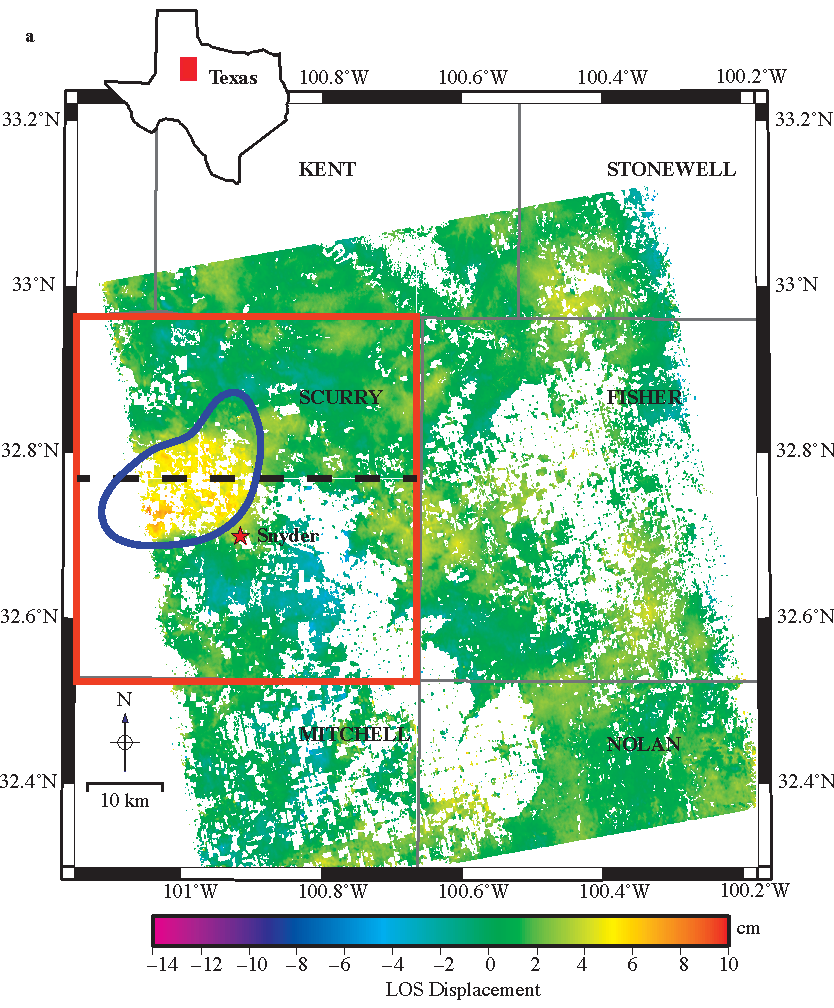
\includegraphics{figs_paper3/Fig1a.pdf}
\label{fig:chpt5_fig1a}
\end{figure}

\clearpage
\begin{figure}
\centering
\includegraphics{figs_paper3/Fig1b.pdf}	
\caption[(a) Total LOS (line of sight) displacement from from January. 08, 2007 to March. 06, 2011. (b) A SAR intensity image of the study area.]{(a) Total LOS (line of sight) displacement from from January. 08, 2007 to March. 06, 2011. (b) A SAR intensity image of the study area.  Red star represents location of the town of Snyder, Texas.  Light grey lines are county boundaries and county names are labeled.  Red lines are the boundaries of our study area, Scurry County.  Blue line is the approximate boundary of the oil field in the study area.  Black dashed line represents location of a profile for surface displacement modeling in the following sections.}
\label{fig:chpt5_fig1b}
\end{figure}

\clearpage
\begin{figure}
	\centering
	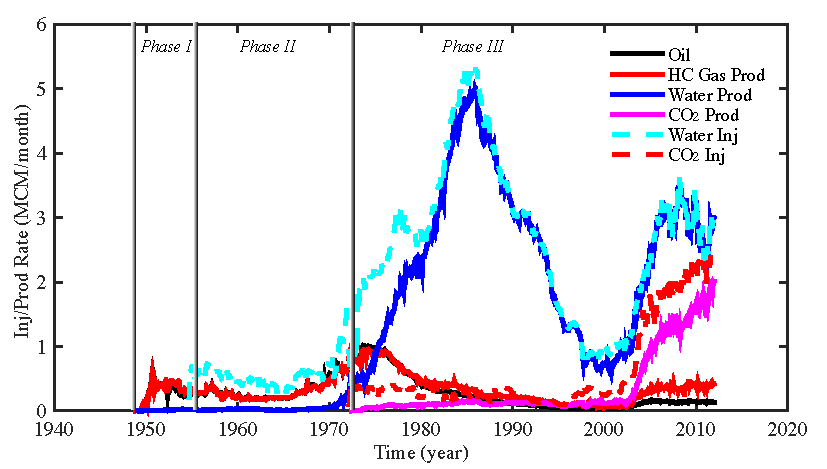
\includegraphics{figs_paper3/Fig2.pdf}	
	\caption[Injection and production history of the study site.]{Injection and production history of the study site.  Phase I is the primary recovery phase.  Phase II is the secondary recovery phase.  Phase III is the tertiary/enhanced oil recovery phases.  Volumes of fluid injection and production are reported at 16 MPa, 41.5 \textordmasculine C (pressure and temperature at reservoir depth). HC is hydrocarbon.}
	\label{fig:chpt5_fig2}
\end{figure}

\clearpage
\begin{figure}
	\centering
	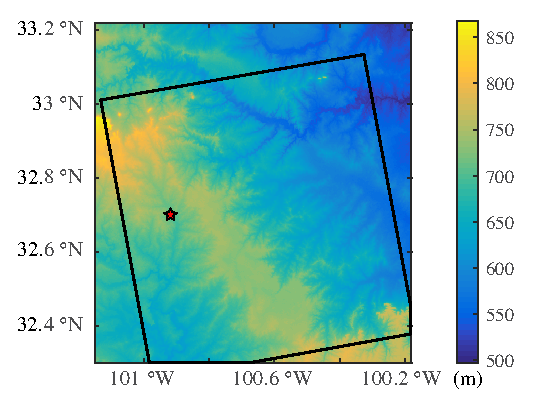
\includegraphics{figs_paper3/Fig3.eps}	
	\caption[DEM of our study area.]{DEM of our study area.  Black lines are the boundaries of the area covered by the interferogram.  Red star represents location of the town Snyder, Texas.}
	\label{fig:chpt5_fig3}
\end{figure}

\clearpage
\begin{figure}
	\centering
	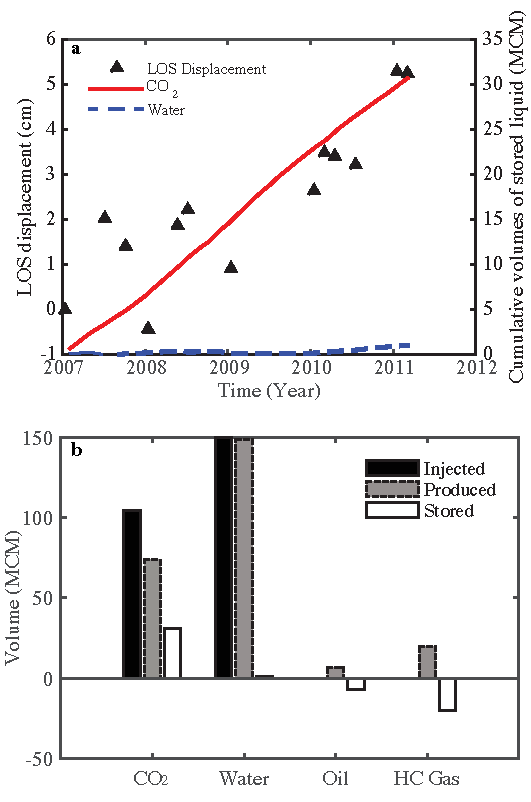
\includegraphics{figs_paper3/Fig4.pdf}	
	\caption[(a) Comparison between Line of Sight (LOS) displacement at Snyder (red star marked in Figure \ref{fig:chpt5_fig1b}) and cumulative volumes of stored (injection minus production) CO$_{2}$ and water in the field from January 2007 to March 2011.  (b) The total volumes of injected/produced/stored CO$_{2}$, water, oil and HC gas in the field from January 2007 – March 2011.]{(a) Comparison between Line of Sight (LOS) displacement at Snyder (red star marked in Figure \ref{fig:chpt5_fig1b}) and cumulative volumes of stored (injection minus production) CO$_{2}$ and water in the field from January 2007 to March 2011.  (b) The total volumes of injected/produced/stored CO$_{2}$, water, oil and HC gas in the field from January 2007 – March 2011.  Volumes of fluid injection and production are reported at 16 MPa, 41.5 \textordmasculine C.}
	\label{fig:chpt5_fig4}
\end{figure}

\clearpage
\begin{figure}
	\centering
	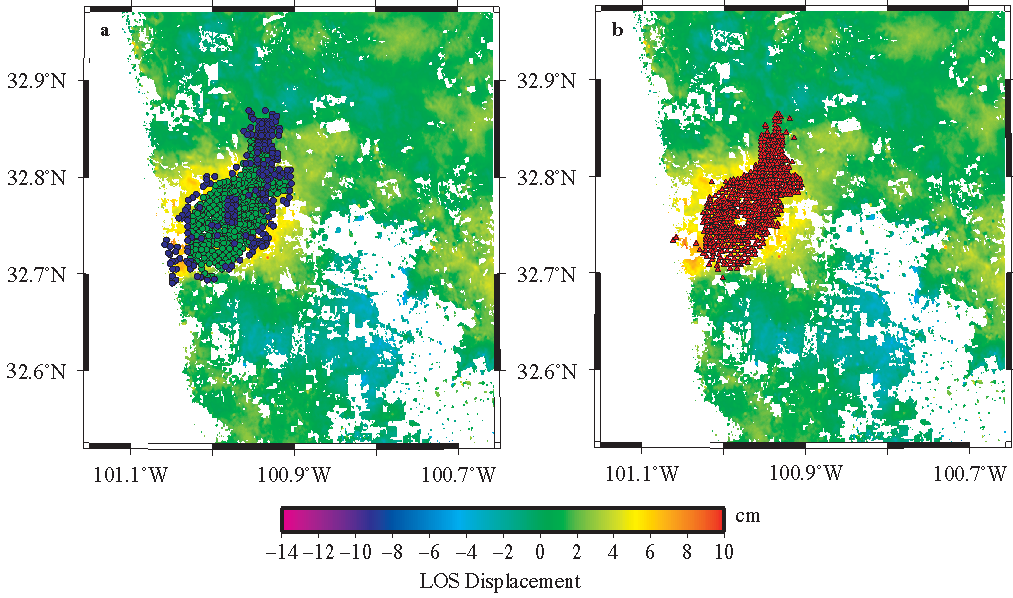
\includegraphics[width=\textwidth]{figs_paper3/Fig5.pdf}	
	\caption{Map of study area, showing total LOS displacement from January 08, 2007 to March. 06, 2011, (a) wells injecting CO$_{2}$ (green circle) and water (blue circle), and (b) well producing CO$_{2}$, water, Oil and HC gas (red triangle).}
	\label{fig:chpt5_fig5}
\end{figure}

\clearpage
\begin{figure}
	\centering
	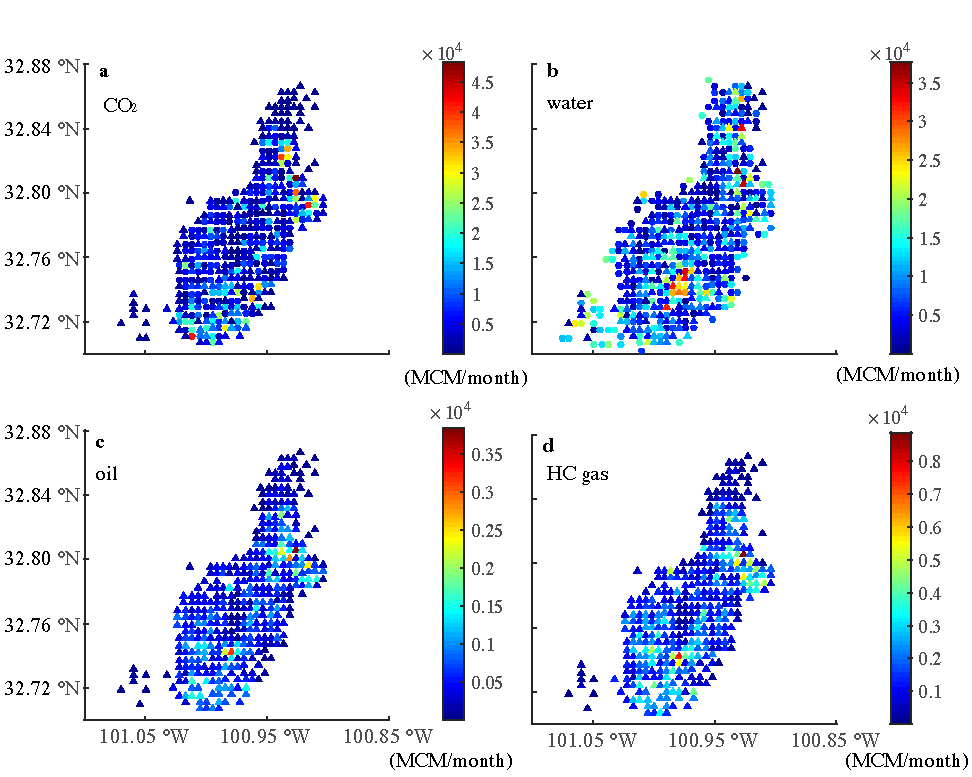
\includegraphics{figs_paper3/Fig6.pdf}	
	\caption[Location of virtual wells for each type fluid and the average monthly injection/production rate for each virtual well.]{Location of virtual wells for each type fluid and the average monthly injection/production rate for each virtual well.  Circles represent injection wells and triangles represent production wells.  Volumes of fluid injection and production are reported at 16 MPa, 41.5 \textordmasculine C.}
	\label{fig:chpt5_fig6}
\end{figure}

\clearpage
\begin{figure}
	\centering
	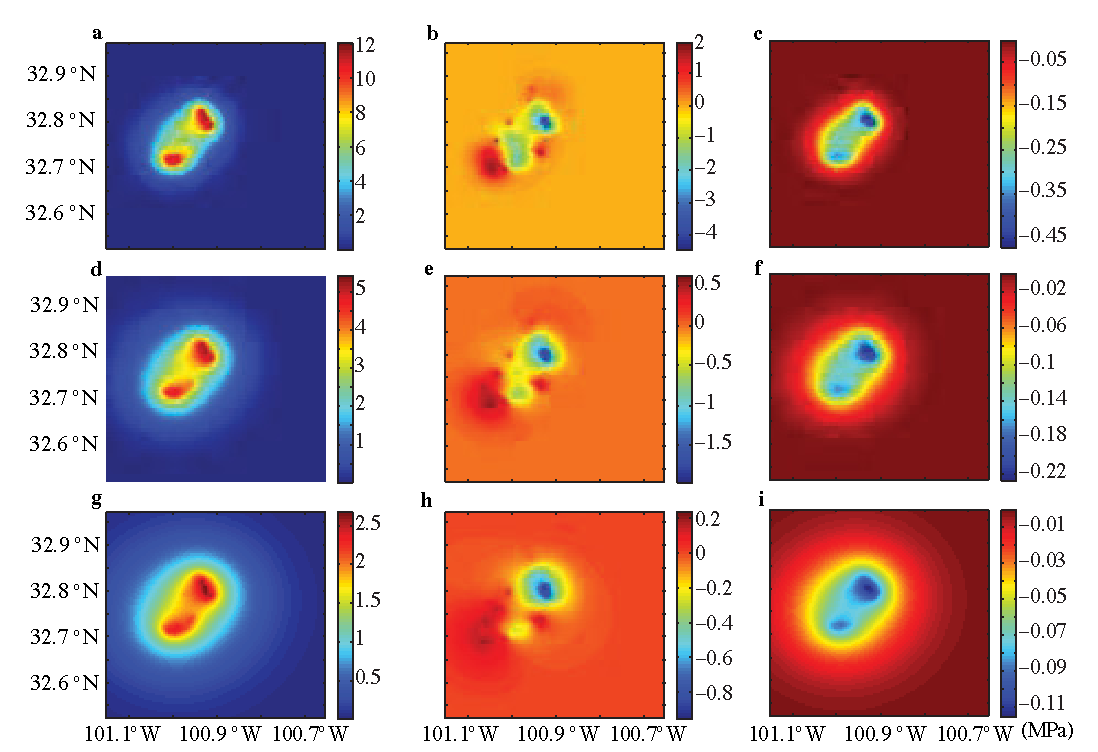
\includegraphics[width=\textwidth]{figs_paper3/Fig7.pdf}	
	\caption[Calculated pressure change due to fluid injection and production at three levels of porosity and permeability.]{Calculated pressure change due to fluid injection and production at three levels of porosity and permeability. (a-c: low porosity/permeability; d-f: medium porosity/permeability; g-i: high porosity and permeability).  a,d and g are calculated pressure buildup due to net CO$_{2}$ injection.  b, e and h are derived from net water injection.  c, f and I are derived from oil and HC gas production}
	\label{fig:chpt5_fig7}
\end{figure}

\clearpage
\begin{figure}
	\centering
	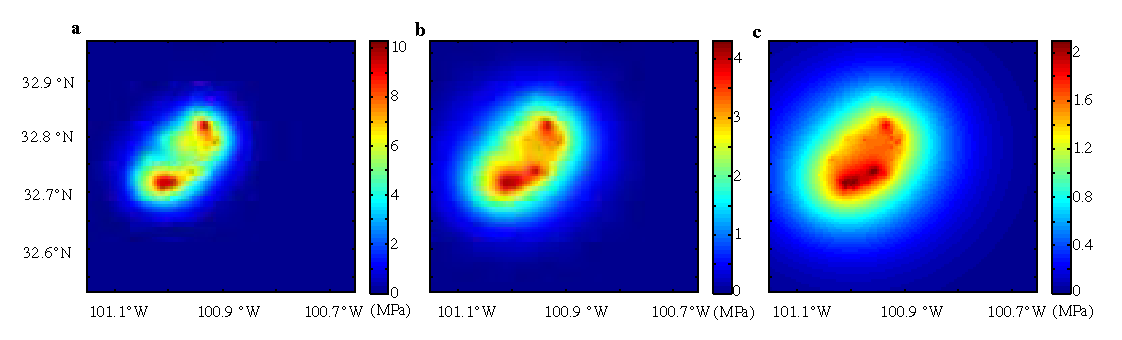
\includegraphics[width=\textwidth]{figs_paper3/Fig8.pdf}	
	\caption[Calculated pressure change due to all injection and production activities at three levels of porosity and permeability.]{Calculated pressure change due to all injection and production activities at three levels of porosity and permeability. (a) low porosity/permeability level; (b) medium porosity/permeability level; (c) high porosity and permeability level.}
	\label{fig:chpt5_fig8}
\end{figure}

\clearpage
\begin{figure}
	\centering
	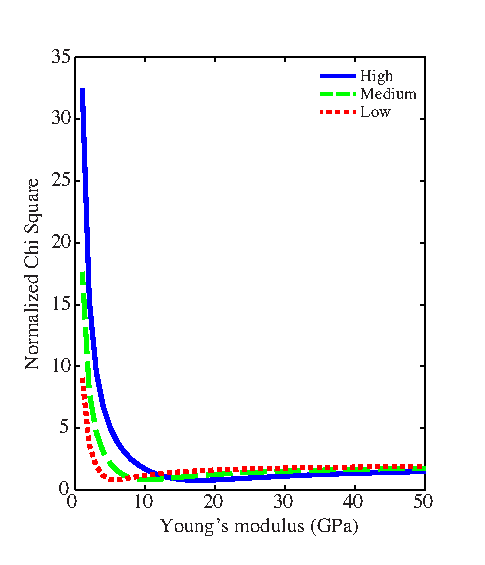
\includegraphics{figs_paper3/Fig9.eps}	
	\caption[Goodness of fit versus Young’s modulus at three levels of pressure change conditions.]{Goodness of fit versus Young’s modulus at three levels of pressure change conditions.  Simulated LOS displacements are fitted to LOS displacement observation along the profile shown in Figure \ref{fig:chpt5_fig1b}.  Note that the minimum value of Young’s modulus is well constrained, but the upper bound value is not.}
	\label{fig:chpt5_fig9}
\end{figure}

\clearpage
\begin{figure}
	\centering
	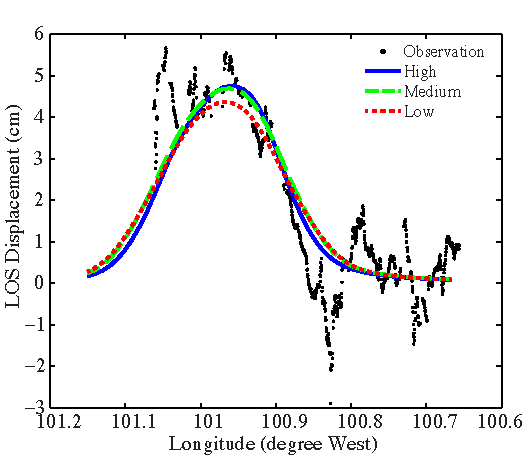
\includegraphics{figs_paper3/Fig10.pdf}	
	\caption{Simulated LOS displacement at three levels of pressure change conditions versus InSAR observation along the profile shown in Figure \ref{fig:chpt5_fig1b}.}
	\label{fig:chpt5_fig10}
\end{figure}

\clearpage
\begin{figure}
	\centering
	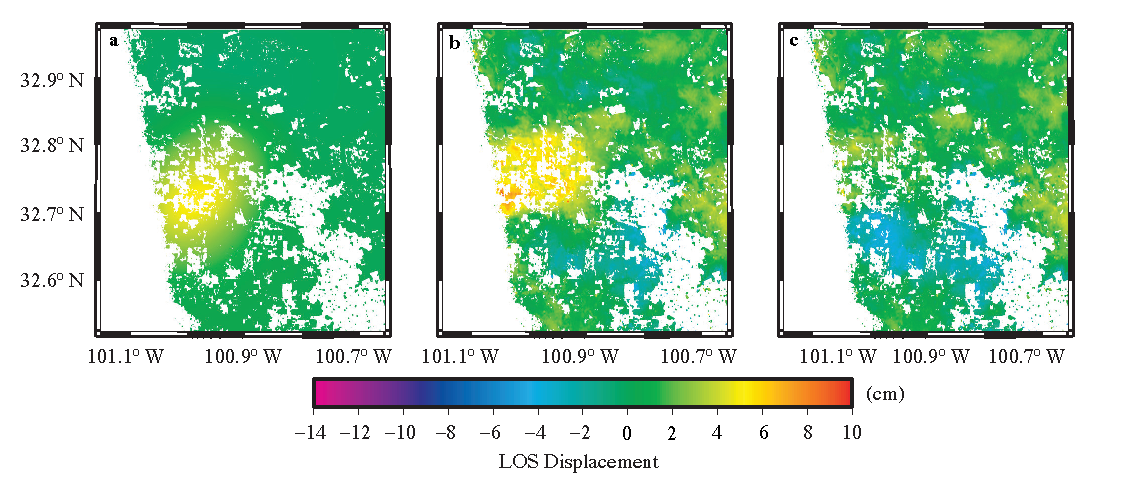
\includegraphics[width=\textwidth]{figs_paper3/Fig11.pdf}	
	\caption[Comparison between simulated LOS displacements and InSAR observation for the entire study area.]{Comparison between simulated LOS displacements and InSAR observation for the entire study area.  Surface displacements were derived from high-pressure change condition.  (a) Simulated LOS displacements; (b) InSAR observation; (c) residual.}
	\label{fig:chpt5_fig11}
\end{figure}
% \end{document}
